\documentclass[journal]{IEEEtran}
\usepackage[T1]{fontenc}
\usepackage{graphicx}
\usepackage{amsmath,amssymb}
\usepackage{booktabs}
\usepackage{multirow}
\usepackage{makecell}
\usepackage{array}
\usepackage[table]{xcolor}
\usepackage{tikz}
\usetikzlibrary{shapes.geometric,arrows.meta,positioning,fit,backgrounds,calc}
\usepackage{algorithm}
\usepackage{algpseudocode}
\usepackage{subcaption}
\usepackage{cite}
\usepackage{url}
\usepackage[hidelinks]{hyperref}
\usepackage{balance}

\definecolor{cpblue}{HTML}{2563EB}
\definecolor{cpgreen}{HTML}{16A34A}
\definecolor{cporange}{HTML}{F59E0B}
\definecolor{cppurple}{HTML}{7C3AED}
\definecolor{cpred}{HTML}{DC2626}
\definecolor{cpgrey}{HTML}{64748B}
\definecolor{rowgrey}{HTML}{F1F5F9}

\algrenewcommand\algorithmicrequire{\textbf{Input:}}
\algrenewcommand\algorithmicensure{\textbf{Output:}}
\makeatletter\newcommand{\tabinput}[1]{\@@input #1 }\makeatother
\newcommand{\tool}[1]{\texttt{\small #1}}

\newcommand{\ToolCount}{105}
\newcommand{\ProjectCount}{65}
\newcommand{\DesignCount}{15}
\newcommand{\PartCount}{608}
\newcommand{\FullOk}{11}
\newcommand{\NoRipOk}{7}
\newcommand{\NetsFull}{455}
\newcommand{\NetsNr}{444}
\newcommand{\NetsAll}{468}
\newcommand{\MedSec}{25.2}
\newcommand{\LayoutPct}{7\,\%}
\newcommand{\DesignPct}{15\,\%}
\newcommand{\TracksPct}{50\,\%}
\newcommand{\MaxLayoutTok}{1{,}900}
\newcommand{\MaxRawTok}{29{,}500}
\newcommand{\SchemaTok}{17{,}400}
\newcommand{\RoutingNote}{All fifteen stored designs are fully routed: the four boards left open here (D10, D12--D14) were completed interactively through longer runs, \tool{optimize\_pcb} placement changes and, for D10, D13 and D14, a few hand-drawn or locked tracks that the router then keeps. D3's copper is entirely hand-drawn (a flexible electrode carrier), so it only checks that kept copper is respected.}


\begin{document}

\title{CircuitPilot: Language Decides, Geometry Guarantees --- An Agent-Operable, Browser-Based Toolchain from Natural Language to Manufacturable Printed Circuit Boards}

\author{Abdelhay~Ali%
\thanks{A.~Ali, e-mail: abdelhay.ali.292@gmail.com.}%
\thanks{Software: \url{https://pcbgo.site}, source: \url{https://github.com/Abdelhayali/CircuitPilot}.}}

\markboth{Preprint, October 2026}{Ali: CircuitPilot --- An Agent-Operable Toolchain for Manufacturable PCBs}

\maketitle

\begin{abstract}
Large language models (LLMs) can read datasheets, choose components and reason about circuits, yet they remain poor at the one thing a printed circuit board (PCB) ultimately is: exact geometry that must pass manufacturing rules. Existing LLM-for-EDA work concentrates on hardware description languages and integrated-circuit flows, and recent PCB efforts address isolated sub-tasks such as schematic generation or benchmark environments. We present \emph{CircuitPilot}, a browser-based schematic-to-fabrication toolchain built around one principle: \emph{the language model decides, the geometric engines guarantee}. The agent expresses intent through \ToolCount{} typed tools exposed over the Model Context Protocol (MCP) and an in-app copilot, while deterministic engines---a negotiated-congestion grid router with blocker discovery, an exact-geometry design-rule checker, distance-field copper pours, a desktop-CNC isolation-milling generator with automatic toolpath verification, a schematic organizer with an orthogonal wire router, and a 3D enclosure kernel---produce outputs that are correct by construction or reported with an actionable reason. One JavaScript engine runs unchanged in the browser, a static web deployment, a Windows application and a headless MCP server. On \DesignCount{} real boards from a wearable biomedical research project (\PartCount{} parts in total), negotiated rip-up raised fully-routed boards from \NoRipOk{} to \FullOk{} and routed \NetsFull{} of \NetsAll{} nets with a median run time of \MedSec{}\,s; compact tool answers cut the state an agent must read to \LayoutPct{} of the raw project for the PCB layout. Isolation-milling jobs for single-sided boards were generated with zero detected shorts or cut nets. We describe the architecture, the algorithms, the agent-oriented tool design, and the limitations that remain.
\end{abstract}

\begin{IEEEkeywords}
Electronic design automation, printed circuit board, large language model agents, Model Context Protocol, maze routing, rip-up and reroute, isolation milling, schematic layout.
\end{IEEEkeywords}

% ============================================================
\section{Introduction}
\IEEEPARstart{A}{} researcher who needs a small custom board---a sensor front end, a wearable node, a test fixture---faces a toolchain built for professional layout engineers. Capable EDA suites such as KiCad~\cite{kicad} are free, but the path from an idea to a board that a fabricator accepts, or that a desktop CNC machine can mill, still requires symbol and footprint management, placement intuition, routing skill, knowledge of design rules, and a separate computer-aided manufacturing (CAM) step~\cite{flatcam,pcb2gcode}. For research groups whose expertise is the application rather than the board, this overhead is repeated for every design iteration.

Large language models appear to be the missing assistant: they read datasheets, recall reference circuits and decompose tasks, and agent frameworks let them act through tools~\cite{yao2023react,schick2023toolformer}. LLM research in electronic design automation has, however, focused mainly on register-transfer-level code and chip design~\cite{chang2023chipgpt,thakur2024verigen,liu2023chipnemo,blocklove2023chipchat,zhong2023llm4eda,pan2025survey} and on analog circuit synthesis~\cite{lai2025analogcoder}. Work specific to PCBs has started only recently and targets individual stages: netlist-to-schematic conversion~\cite{matsuo2025schemato}, schematic generation~\cite{luo2026schgen}, question answering~\cite{srinivasan2026pcbqa}, and benchmark environments for layout~\cite{song2026pcbworld,lu2026omnilayout}. The central difficulty is unchanged: a PCB is a geometric object that must satisfy hundreds of clearance, width, drill and edge constraints exactly, and a language model that emits coordinates directly cannot be trusted to satisfy them.

\textbf{Problem.} How can a language-model agent take a design from a sentence to a manufacturable board---fabrication files for a PCB service, or G-code for a desktop CNC---without the model ever being responsible for geometric correctness, and without the user installing or learning a professional EDA tool?

\textbf{Approach.} We split responsibilities. The agent makes the decisions that need knowledge and judgment: which parts, how they connect, which nets are power, where connectors and antennas go, which design-rule preset suits the process. Deterministic engines turn those decisions into geometry and verify it. Every engine answers the agent in compact, structured text, and every failure carries a reason that names the obstacle and a next step. We call this principle \emph{language decides, geometry guarantees}.

\textbf{Motivating story.} CircuitPilot grew out of a human-body-communication (HBC) electrocardiogram (ECG) wearable project in which one researcher needed dozens of board variants---transmitter and receiver nodes on different microcontrollers, coin-cell and round form factors, test panels, flexible electrode leads, and single-sided boards milled on a desktop CNC. The tool's own project database holds \ProjectCount{} such designs. Iterating at that rate with a conventional flow was impractical. The benchmark in Section~\ref{sec:eval} is drawn from these designs, so every result reflects a real board rather than a synthetic netlist.

\textbf{Contributions.}
\begin{enumerate}
\item \emph{An agent-operable EDA architecture} in which a single JavaScript engine serves the browser editor, a static web deployment, a Windows application and a headless MCP~\cite{anthropic2024mcp,mcpspec} server, exposing \ToolCount{} typed tools (Section~\ref{sec:arch}).
\item \emph{Six design principles for agent-facing EDA tools}: compact filtered state, actionable failure reasons, one-call recipes, background jobs, version safety and visual self-checks. We measure the first (Section~\ref{sec:tools}).
\item \emph{A negotiated-congestion grid router for PCBs} that combines windowed weighted A*, a bidirectional reachability filter, soft-mode blocker discovery, history costs, rip-up of the cheapest blockers, geometry straightening and exact-geometry repair (Algorithm~\ref{alg:route}).
\item \emph{A verified desktop-CNC fabrication path}: isolation toolpaths from exact Euclidean distance transforms, an automatic check for shorts and cut nets, optional SMD-pad thermal relief, and 2D/3D previews of the milled board (Algorithm~\ref{alg:cnc}).
\item \emph{A readable-schematic organizer} with an orthogonal maze wire router that keeps different nets from overlapping (Algorithm~\ref{alg:org}).
\item \emph{An evaluation on \DesignCount{} real boards}, with an ablation of rip-up and reroute, CNC statistics and tool-answer sizes. The benchmark scripts are released with the tool.
\end{enumerate}

% ============================================================
\section{Related Work}
\label{sec:related}

\textbf{Routing.} Maze routing goes back to Lee's wave expansion~\cite{lee1961}, built on shortest-path search~\cite{dijkstra1959}. It was accelerated by Hadlock's detour-number search~\cite{hadlock1977} and by heuristic A* search~\cite{hart1968}, while Hightower's line search~\cite{hightower1969} avoided the grid. Sequential routers depend on net order. Rip-up and reroute~\cite{dees1982} and iterative global wiring~\cite{nair1987} mitigate this, and PathFinder's negotiated congestion~\cite{mcmurchie1995} turned it into a principled cost scheme; Kahng \emph{et al.}~\cite{kahng2011} survey these methods. Freerouting~\cite{freerouting} is the router most used with open PCB tools. Learning-based placement and routing have shown promise for chips~\cite{mirhoseini2021}, for PCB placement~\cite{vassallo2024} and for circuit routing~\cite{he2022}. Our router borrows negotiation from PathFinder and adds blocker discovery and agent-readable failure explanations.

\textbf{LLMs for EDA and PCBs.} Surveys~\cite{zhong2023llm4eda,pan2025survey} document rapid progress in HDL generation~\cite{chang2023chipgpt,thakur2024verigen}, domain adaptation~\cite{liu2023chipnemo}, conversational hardware design~\cite{blocklove2023chipchat} and analog synthesis~\cite{lai2025analogcoder}. For boards, Schemato converts netlists to schematics~\cite{matsuo2025schemato}, SchGen generates PCB schematics~\cite{luo2026schgen}, PCB-QA evaluates PCB design knowledge~\cite{srinivasan2026pcbqa}, and PCBWorld and OmniLayout provide layout benchmarks~\cite{song2026pcbworld,lu2026omnilayout}. These works study individual stages or evaluate models; CircuitPilot is an end-to-end system in which the model never produces geometry itself.

\textbf{Tool-using agents.} ReAct interleaves reasoning and acting~\cite{yao2023react}, and Toolformer learns when to call tools~\cite{schick2023toolformer}. MCP standardizes how agents discover and call external tools~\cite{anthropic2024mcp,mcpspec}, and its security landscape has been surveyed~\cite{hou2026mcp}. We contribute design guidance for tools whose results are large geometric states.

\textbf{Schematic drawing and milling.} Automatic schematic generation dates to the 1980s~\cite{arya1985} and draws on layered~\cite{sugiyama1981} and orthogonal~\cite{tamassia1987} graph drawing. PCB isolation milling is established for prototyping~\cite{sterian2001}, with FlatCAM~\cite{flatcam} and pcb2gcode~\cite{pcb2gcode} converting Gerber files~\cite{gerber2026} into G-code as a separate step.

Table~\ref{tab:position} positions CircuitPilot against these lines of work.

\begin{table}[t]
\centering
\caption{Scope of CircuitPilot relative to related lines of work.}
\label{tab:position}
\footnotesize
\setlength{\tabcolsep}{2.5pt}
\rowcolors{2}{rowgrey}{white}
\begin{tabular}{@{}lccccc@{}}
\toprule
 & \makecell{NL\\input} & \makecell{Sch-\\ematic} & \makecell{Place\\+route} & \makecell{Fab files\\(Gerber)} & \makecell{CNC G-code\\+ enclosure} \\
\midrule
KiCad + Freerouting~\cite{kicad,freerouting} & -- & \checkmark & \checkmark & \checkmark & -- \\
FlatCAM, pcb2gcode~\cite{flatcam,pcb2gcode} & -- & -- & -- & input & G-code \\
LLM-for-HDL~\cite{chang2023chipgpt,thakur2024verigen} & \checkmark & -- & -- & -- & -- \\
Schemato, SchGen~\cite{matsuo2025schemato,luo2026schgen} & \checkmark & \checkmark & -- & -- & -- \\
PCBWorld, OmniLayout~\cite{song2026pcbworld,lu2026omnilayout} & \checkmark & bench. & bench. & -- & -- \\
\textbf{CircuitPilot (ours)} & \checkmark & \checkmark & \checkmark & \checkmark & \checkmark \\
\bottomrule
\end{tabular}
\vspace{-2mm}
\end{table}

% ============================================================
\section{System Architecture}
\label{sec:arch}

Fig.~\ref{fig:arch} shows the architecture. The design model is one JSON document: components with symbol, footprint and supplier data; named nets of \texttt{REF.PIN} references; the board outline; and the PCB state (placements, tracks, vias, pours, keep-outs, holes, text), together with design rules and the enclosure. Every editing operation is a function of the shared \emph{engine} (about 540\,kB of plain JavaScript, with no build step) that mutates this document inside a checkpointed transaction.

\begin{figure*}[t]
\centering
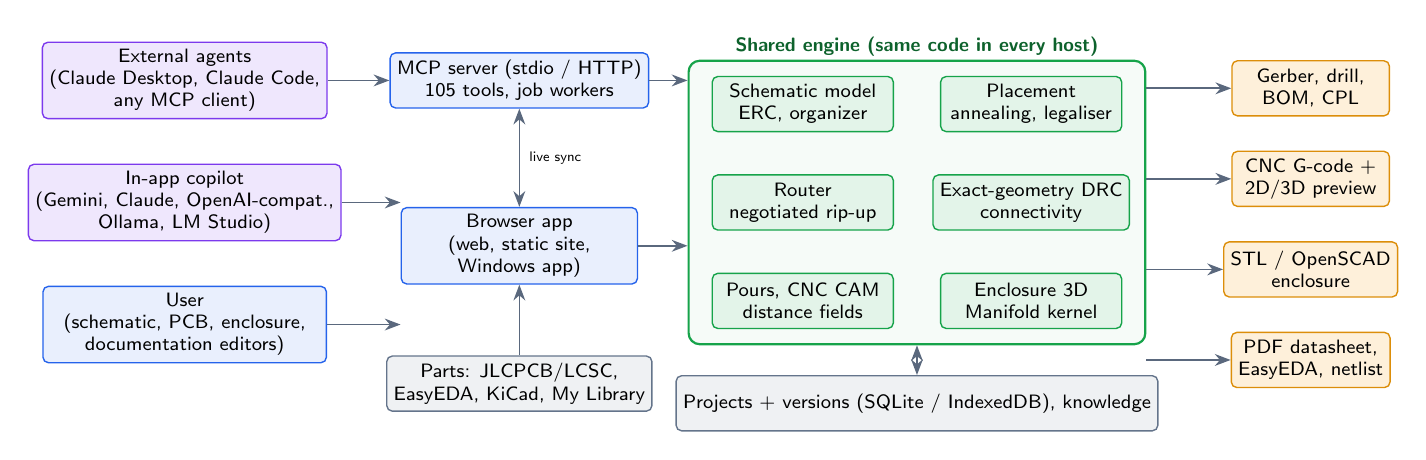
\begin{tikzpicture}[
  font=\sffamily\scriptsize, >=Stealth,
  box/.style={draw, rounded corners=2pt, align=center, minimum height=7mm, inner sep=2.5pt, line width=0.5pt},
  agent/.style={box, fill=cppurple!12, draw=cppurple},
  ui/.style={box, fill=cpblue!10, draw=cpblue},
  eng/.style={box, fill=cpgreen!12, draw=cpgreen, minimum width=23mm},
  outn/.style={box, fill=cporange!15, draw=cporange!90!black, minimum width=20mm},
  data/.style={box, fill=cpgrey!10, draw=cpgrey},
  arr/.style={->, line width=0.6pt, draw=cpgrey!90!black}]
% agents
\node[agent, minimum width=36mm] (ext) at (0,2.1) {External agents\\(Claude Desktop, Claude Code,\\any MCP client)};
\node[agent, minimum width=36mm] (cop) at (0,0.55) {In-app copilot\\(Gemini, Claude, OpenAI-compat.,\\Ollama, LM Studio)};
\node[ui, minimum width=36mm] (user) at (0,-1.0) {User\\(schematic, PCB, enclosure,\\documentation editors)};
% interfaces
\node[ui, minimum width=30mm] (mcp) at (4.25,2.1) {MCP server (stdio / HTTP)\\\ToolCount{} tools, job workers};
\node[ui, minimum width=30mm] (app) at (4.25,0.0) {Browser app\\(web, static site,\\Windows app)};
\node[data, minimum width=30mm] (db) at (4.25,-1.75) {Parts: JLCPCB/LCSC,\\EasyEDA, KiCad, My Library};
% engine
\node[draw=cpgreen, line width=0.8pt, rounded corners=4pt, fill=cpgreen!4, minimum width=58mm, minimum height=36mm] (E) at (9.3,0.55) {};
\node[font=\sffamily\scriptsize\bfseries, text=cpgreen!60!black] at (9.3,2.53) {Shared engine (same code in every host)};
\node[eng] (sch) at (7.85,1.8) {Schematic model\\ERC, organizer};
\node[eng] (pl) at (10.75,1.8) {Placement\\annealing, legaliser};
\node[eng] (rt) at (7.85,0.55) {Router\\negotiated rip-up};
\node[eng] (drc) at (10.75,0.55) {Exact-geometry DRC\\connectivity};
\node[eng] (pour) at (7.85,-0.7) {Pours, CNC CAM\\distance fields};
\node[eng] (enc) at (10.75,-0.7) {Enclosure 3D\\Manifold kernel};
\node[data, minimum width=58mm] (proj) at (9.3,-2.0) {Projects + versions (SQLite / IndexedDB), knowledge};
% outputs
\node[outn] (o1) at (14.3,2.0) {Gerber, drill,\\BOM, CPL};
\node[outn] (o2) at (14.3,0.85) {CNC G-code +\\2D/3D preview};
\node[outn] (o3) at (14.3,-0.3) {STL / OpenSCAD\\enclosure};
\node[outn] (o4) at (14.3,-1.45) {PDF datasheet,\\EasyEDA, netlist};
% arrows
\draw[arr] (ext) -- (mcp);
\draw[arr] (cop.east) -- (app.west |- cop.east);
\draw[arr] (user.east) -- (app.west |- user.east);
\draw[arr] (mcp.east) -- (E.west |- mcp.east);
\draw[arr] (app.east) -- (E.west |- app.east);
\draw[arr, <->] (mcp.south) -- node[right, font=\sffamily\tiny]{live sync} (app.north);
\draw[arr] (db) -- (app);
\draw[arr, <->] (proj.north) -- (E.south);
\foreach \o in {o1,o2,o3,o4} \draw[arr] (E.east |- \o) -- (\o.west);
\end{tikzpicture}
\caption{CircuitPilot architecture. Agents (purple) and the user act through the MCP server or the browser app (blue). Both call the same engine (green), which produces fabrication outputs (orange). Long operations run in worker threads; projects are versioned, so an agent's change can be undone.}
\label{fig:arch}
\end{figure*}

\textbf{Hosts.} The same engine files run in four hosts. (i)~The browser app talks to a small Python server (projects and parts databases in SQLite, proxy to supplier APIs). (ii)~A static deployment on GitHub Pages replaces the server with an in-browser backend: projects in IndexedDB, and part search through a stateless relay worker. (iii)~A Windows application bundles the server. (iv)~The MCP server loads the engine into a Node.js \texttt{vm} context and runs long operations (routing, optimisation, export) in worker threads, returning a job identifier that the agent polls. Edits made through MCP are saved to the same project store and appear live in an open browser tab, so a human can watch and intervene.

\textbf{Agents.} Two kinds of agent use the tools. External agents (Claude Desktop, Claude Code, any MCP client) call the \ToolCount{} MCP tools. The in-app copilot uses the 88 engine tools with a model of the user's choice: Gemini~\cite{gemini2023}, Claude, OpenAI-compatible endpoints, Ollama or LM Studio. In both cases the model never edits coordinates directly unless it calls an explicit geometric tool such as \tool{add\_track}, and even then the result is checked.

\textbf{Parts.} Part search covers the JLCPCB/LCSC catalogue, with symbols and footprints from the official EasyEDA library, plus KiCad footprints and a user library. \tool{get\_part} returns the exact pinout and footprint, so the agent wires pins by name instead of guessing.

\subsection{Tool Interface}
\label{sec:tools}

Table~\ref{tab:tools} groups the tools. They follow six principles derived from watching agents fail.

\begin{table}[t]
\centering
\caption{The \ToolCount{} MCP tools by category (examples).}
\label{tab:tools}
\footnotesize
\setlength{\tabcolsep}{3pt}
\rowcolors{2}{rowgrey}{white}
\begin{tabular}{@{}lc>{\raggedright\arraybackslash}p{47mm}@{}}
\toprule
Category & \# & Examples \\
\midrule
Project, versions, jobs & 14 & \tool{open\_project}, \tool{restore\_project\_version}, \tool{job\_status}, \tool{batch} \\
Parts, knowledge, web & 19 & \tool{search\_parts}, \tool{get\_part}, \tool{create\_part}, \tool{knowledge\_search} \\
Schematic & 13 & \tool{add\_components}, \tool{connect}, \tool{run\_erc}, \tool{organize\_schematic} \\
Board and placement & 14 & \tool{generate\_pcb}, \tool{place\_in\_free\_area}, \tool{optimize\_pcb} \\
Routing and copper & 16 & \tool{route\_pcb}, \tool{reroute}, \tool{add\_via}, \tool{connect\_pads\_to\_pour} \\
Rules and verification & 5 & \tool{set\_design\_rules}, \tool{run\_drc}, \tool{view\_design} \\
Silkscreen, documentation & 8 & \tool{arrange\_silk\_labels}, \tool{set\_documentation} \\
Enclosure & 9 & \tool{set\_enclosure\_script}, \tool{check\_enclosure} \\
Fabrication and quotes & 7 & \tool{export\_gerbers}, \tool{export\_cnc\_gcode}, \tool{jlcpcb\_quote} \\
\bottomrule
\end{tabular}
\vspace{-2mm}
\end{table}

\begin{itemize}\setlength{\itemsep}{1pt}
\item[] \textbf{P1 Compact, filterable state.} Answers are summaries rather than the raw document: \tool{get\_pcb\_layout} lists parts and pads, filtered by reference or region; \tool{run\_drc} returns five violations unless \texttt{full} is set; \tool{get\_tracks} accepts \texttt{near} and \texttt{region}.
\item[] \textbf{P2 Actionable failures.} When a net cannot be routed, the router names the pads it could not join, what surrounds them (neighbouring pins, kept copper, keep-outs, the board edge) and whether a via fits beside the pad, and it suggests a next tool (Section~\ref{sec:router}).
\item[] \textbf{P3 One-call recipes.} Expert sequences are single tools. \tool{reroute}, for example, removes pours and autorouted copper, routes the power nets first, then the rest, restores the pours, adds stitching vias, tidies the silkscreen and runs DRC.
\item[] \textbf{P4 Background jobs.} Operations that take minutes return a job identifier, so the MCP session never times out.
\item[] \textbf{P5 Version safety.} Every save is versioned and the copilot checkpoints each turn, so a wrong agent action can be undone.
\item[] \textbf{P6 Visual self-check.} \tool{view\_design} returns a rendered image of the schematic, PCB, 3D board or enclosure, so a multimodal agent can inspect its own result.
\end{itemize}

Fig.~\ref{fig:flow} shows the typical agent loop these tools support.

\begin{figure}[t]
\centering
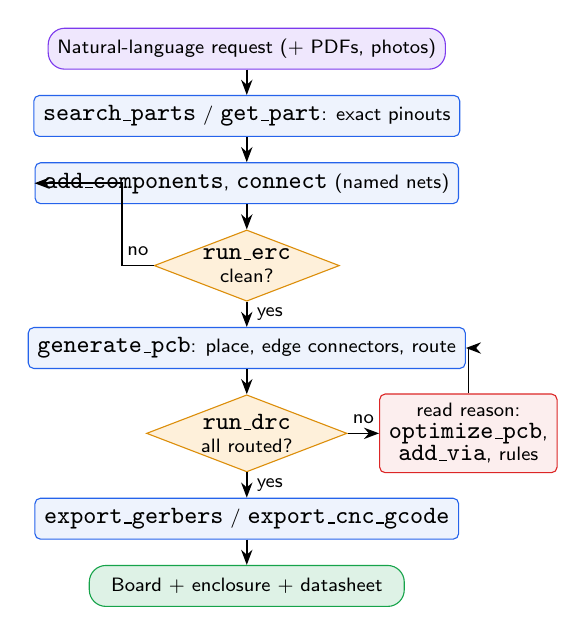
\begin{tikzpicture}[font=\sffamily\scriptsize, >=Stealth, node distance=3.2mm,
  st/.style={draw, rounded corners=2pt, fill=cpblue!8, draw=cpblue, minimum width=40mm, minimum height=5.2mm, align=center},
  dec/.style={draw, diamond, aspect=2.6, fill=cporange!15, draw=cporange!90!black, inner sep=0.6pt, align=center},
  term/.style={draw, rounded corners=6pt, fill=cppurple!12, draw=cppurple, minimum width=40mm, minimum height=5.2mm, align=center},
  ok/.style={draw, rounded corners=6pt, fill=cpgreen!14, draw=cpgreen, minimum width=40mm, minimum height=5.2mm, align=center},
  arr/.style={->, line width=0.55pt}]
\node[term] (a) {Natural-language request (+ PDFs, photos)};
\node[st, below=of a] (b) {\tool{search\_parts} / \tool{get\_part}: exact pinouts};
\node[st, below=of b] (c) {\tool{add\_components}, \tool{connect} (named nets)};
\node[dec, below=of c] (d) {\tool{run\_erc}\\clean?};
\node[st, below=of d] (e) {\tool{generate\_pcb}: place, edge connectors, route};
\node[dec, below=of e] (f) {\tool{run\_drc}\\all routed?};
\node[st, below=of f] (g) {\tool{export\_gerbers} / \tool{export\_cnc\_gcode}};
\node[ok, below=of g] (h) {Board + enclosure + datasheet};
\node[st, right=4mm of f, minimum width=17mm, fill=cpred!8, draw=cpred] (fix) {read reason:\\\tool{optimize\_pcb},\\\tool{add\_via}, rules};
\draw[arr] (a)--(b); \draw[arr] (b)--(c); \draw[arr] (c)--(d);
\draw[arr] (d)--node[right]{yes}(e); \draw[arr] (e)--(f); \draw[arr] (f)--node[right]{yes}(g); \draw[arr] (g)--(h);
\draw[arr] (d.west) -- node[above]{no} ++(-4mm,0) |- (c.west);
\draw[arr] (f.east) -- node[above]{no} (fix.west);
\draw[arr] (fix.north) |- (e.east);
\end{tikzpicture}
\caption{Typical agent loop. ERC and DRC gate each stage; a failed route returns a reason that maps to a next tool rather than a bare ``unrouted''.}
\label{fig:flow}
\vspace{-3mm}
\end{figure}

% ============================================================
\section{Algorithms}
\label{sec:alg}

\subsection{Placement}
\texttt{generate\_pcb} places connectors on the nearest board edge (USB, jacks and RF facing outward), then places the remaining parts by a connectivity-driven constructive pass followed by simulated annealing on half-perimeter wire length (HPWL), with the courtyard spacing kept by a legaliser. \tool{optimize\_pcb} repeats annealing with extra room around the parts of failing nets, routes each candidate, and keeps the best result. It can also shrink the board step by step while every net still routes.

\subsection{Negotiated-Congestion Grid Router}
\label{sec:router}

\textbf{Grid and obstacles.} The board is rasterised at pitch $g=\min(0.25, \max(0.05, \lfloor m/0.05\rfloor\,0.025))$\,mm, where $m$ is the smallest trace width or clearance; $g$ is increased until the grid has at most $1.5\times10^6$ cells per layer. For each trace width $w$, a cell is blocked for a net if its centre lies within $w/2 + c + \delta$ of copper belonging to another net, where $c$ is the applicable clearance (pad, via, hole or edge) and $\delta=\max(0.01, 0.1g)$\,mm is a safety margin against rounding. Separate via maps enforce via-to-copper and hole-to-hole clearance. The obstacle maps hold counts that are updated incrementally when copper is added or ripped up, so the map for one net is ``counts minus its own contribution'', built in a single linear pass.

\textbf{Search.} Each two-terminal connection is a weighted A*~\cite{hart1968} search over (layer, cell) states with eight neighbours (four in 90\textdegree{} mode). The cost of a step from cell $u$ to $v$ is
\begin{equation}
c(u,v) = \ell(u,v) + \tau\,[\text{turn}] + h_v + \sigma\,[\text{soft}\wedge v\in\mathcal{O}] ,
\end{equation}
with step length $\ell\in\{1,\sqrt2\}$, turn penalty $\tau=0.6$, history cost $h_v$, and soft-mode penalty $\sigma=3$ for crossing copper of other routed nets ($\mathcal{O}$). A layer change costs $\max(8, 2.5/g)$. The heuristic is the octile distance to the nearest target pad, weighted by $1.15$. The search runs first inside the bounding box of the tree and the target, enlarged by 8\,mm, and then on the whole board. On large windows a bidirectional breadth-first flood from the source tree and the target first tests whether a path exists at all; because a blocked terminal is usually boxed in, this rejects hopeless searches in far fewer expansions than A*.

\textbf{Multi-terminal nets.} Pads already joined by kept copper form islands. A net grows like Prim's algorithm: it starts from the largest island nearest the centroid and repeatedly connects the nearest remaining island to the whole current tree. When a connection does not fit at the net's width, narrower widths are tried if neck-down is allowed. Each committed path is straightened: from every point the farthest point reachable by one clear 0/45/90\textdegree{} segment, or by a two-leg elbow, replaces the grid staircase, and the cells are re-rasterised from the straightened geometry.

\textbf{Negotiation.} Algorithm~\ref{alg:route} summarises the rip-up loop. It differs from PathFinder~\cite{mcmurchie1995} in two ways. First, \emph{blocker discovery}: a failed net is routed once in soft mode, where other nets' copper is passable at a cost, which reveals the specific nets in its way. Second, \emph{selective rip-up}: only the two to four cheapest blockers are removed, ranked by pad count, HPWL and how often they have already been ripped. The probe path also raises the history cost of its corridor, so later searches by other nets avoid it. Moves are accepted when the score $S = 10^7 F + L + 1.5V$ improves ($F$ failed nets, $L$ track length, $V$ vias), and equal-failure moves are accepted with probability $0.3$ to escape plateaus. After 25 moves without improvement the router restarts from the best state with the failed nets ordered first.

\textbf{Exact-geometry closure.} The grid is an approximation, so two passes follow. Connectivity is recomputed from exact geometry (tracks, vias and pours), and any net found broken---typically a pour split into islands---is routed again with the live pour as part of its source tree. Then DRC is run, nets with clearance violations are re-routed with an extra 0.04\,mm margin, and the repair is kept only if it does not lose connectivity. Nets still open receive the explanation described in principle~P2.

\begin{algorithm}[t]
\caption{Negotiated rip-up and reroute with blocker discovery}
\label{alg:route}
\small
\begin{algorithmic}[1]
\Require nets $\mathcal{N}$, placement, rules, time budget $T$
\Ensure tracks, vias, open nets with reasons
\State build obstacle-count maps; $h \gets 0$
\State route all nets in ascending HPWL order; $B \gets$ snapshot
\If{some nets failed} rip all; route failed nets first; keep the better result \EndIf
\While{failed nets exist \textbf{and} time $< T$}
  \State pick a failed net $f$ at random; rip $f$
  \State $(P,\mathcal{K}) \gets$ \Call{RouteSoft}{$f$} \Comment{path, blockers}
  \State $h_v \gets \min(8, h_v + 0.4)$ for $v$ in the halo of $P$
  \If{$P=\varnothing$} mark $f$ hard (or allow via-in-pad); \textbf{continue} \EndIf
  \State $\mathcal{K} \gets$ 2--4 cheapest of $\mathcal{K}$ (pads, HPWL, rip count)
  \State rip $\mathcal{K}$; route $f$; route $\mathcal{K}$ (most-ripped first)
  \State retry any net of $\mathcal{K}\cup\{f\}$ still failing
  \If{$S$ improved \textbf{or} (no new failure \textbf{and} rand $<0.3$)} accept; update $B$ if best
  \Else{} restore \EndIf
  \If{25 moves without improvement} restore $B$; restart with failed nets first \EndIf
\EndWhile
\State restore $B$; reconnect nets broken in exact geometry (pour islands)
\State DRC repair with $+0.04$\,mm margin; explain open nets
\end{algorithmic}
\end{algorithm}

\subsection{Copper Pours and SMD Pad Relief}
A pour is filled on a raster as a signed distance field: obstacles (other nets' copper grown by the pour clearance, keep-outs, board-edge clearance, drill holes) are subtracted, small or orphaned islands are removed, and the boundary is traced into polygons. With \texttt{smdPadRelief}, each SMD pad of the pour net is surrounded by a clearance gap crossed by four spokes, so a hand-soldered pad does not sink its heat into the plane. On a CNC-milled board this also leaves a visible solder spot on each pad instead of plain copper.

\subsection{Desktop-CNC Isolation Milling}
Algorithm~\ref{alg:cnc} converts the routed single-sided board into G-code for a GRBL desktop mill without an intermediate Gerber or CAM tool. Copper is painted on a fine raster ($g = 0.02$\,mm in our runs), and an exact Euclidean distance transform~\cite{felzenszwalb2012} gives the distance from every node to the copper. Isolation rings are iso-contours of this field at $d_k = \phi/2 + k\,\phi(1-o)$, where $\phi$ is the groove width of the V-bit at the chosen depth ($\phi = t + 2z\tan(\alpha/2)$ for tip $t$, depth $z$ and angle $\alpha$) and $o$ is the overlap between passes. Contours are extracted by oriented marching squares~\cite{lorensen1987}, simplified, and oriented for conventional milling. Before writing files, the generator \emph{verifies the toolpath}. It labels the connected copper regions, then labels the copper grown to the narrowest groove the bit could cut; two nets in one grown region would be shorted. Labelling the copper remaining after the widest groove detects nets that the cutter would sever. Copper that the pour leaves out (under SMD parts, in keep-outs) is cleared by zig-zag passes so that no floating slivers remain. Drill files are grouped by bit size, and the board cutout uses an end mill with holding tabs. The same toolpaths are rendered as the milled result in 2D and as a textured, bump-mapped 3D model, so the user can inspect the board before cutting copper.

\begin{algorithm}[t]
\caption{Verified isolation toolpaths}
\label{alg:cnc}
\small
\begin{algorithmic}[1]
\Require copper of the milled layer, V-bit $(t,\alpha,z)$, passes $K$, overlap $o$
\Ensure isolation, drill and cutout G-code; 2D/3D previews
\State $\phi \gets t + 2z\tan(\alpha/2)$; mirror if parts go on the bare side
\State paint copper mask $C$ and board mask on a grid of pitch $g$
\State $D \gets$ \Call{EDT}{$C$} \Comment{exact Euclidean distance}
\For{$k=0\ldots K-1$} $R_k \gets$ \Call{MarchingSquares}{$D - \phi/2 - k\phi(1-o)$} \EndFor
\State $L_C \gets$ \Call{Label}{$C$}; $L_n \gets$ \Call{Label}{$D \le \phi_{\min}/2$}
\State \textbf{if} a region of $L_n$ holds two nets \textbf{then} report short
\State \textbf{if} a net splits after the widest groove \textbf{then} report cut net
\State clear pour-free areas (zig-zag); simplify and order paths
\State emit G-code: isolation, drills per bit, cutout with tabs
\end{algorithmic}
\end{algorithm}

\subsection{Schematic Organizer and Wire Router}
Agents place symbols poorly: they put parts in arbitrary grid positions and connect them with long crossing wires or with net labels that hide the circuit's structure. The organizer (Algorithm~\ref{alg:org}) rebuilds the drawing in the style of a hand-drawn schematic. Integrated circuits and modules form a row; every small part is assigned by breadth-first search over signal nets to the host pin it serves, and is placed beside that pin, continuing outward along chains. Rotation follows conventions: a part on ground stands vertically with ground at the bottom, a part on a supply stands vertically with the supply on top, series parts lie horizontally, and decoupling capacitors attach to supply-named pins. Wires are then routed by a Dijkstra search~\cite{dijkstra1959} on a 10-unit grid whose state is (cell, direction): each step costs 1, a bend costs 4, crossing another net costs 8, and running along another net's wire, through a symbol, a power symbol or a net label, or through an unconnected pin end is forbidden. Junction dots appear where three or more wire ends meet, and each net name is placed on its longest horizontal run. This follows the orthogonal-drawing tradition~\cite{tamassia1987} with a router in place of an embedding.

\begin{algorithm}[t]
\caption{Schematic organizer}
\label{alg:org}
\small
\begin{algorithmic}[1]
\Require symbols, nets
\Ensure positions, rotations, orthogonal wires
\State main parts $M \gets$ ICs and modules, chained by shared nets
\State owner$(p) \gets$ BFS from $M$ over signal nets (paired 2-pin parts first)
\For{each small part $p$ in BFS order}
  \State rotation by role: GND $\downarrow$, supply $\uparrow$, series $\leftrightarrow$
  \State place beside owner pin; candidates scored by outward $+1.6\cdot$lateral
\EndFor
\State lay clusters out left to right (wrap); centre
\State \Call{MazeRoute}{nets by span}: Dijkstra over (cell, dir), bend 4, cross 8
\end{algorithmic}
\end{algorithm}

\subsection{Enclosure}
An enclosure is either a parametric box or a script in a small modelling language evaluated by the Manifold geometry kernel~\cite{manifold} (WebAssembly), with a BSP fallback. It is built around the board's 3D model, with cut-outs for edge connectors, standoffs at mounting holes, and printability checks (wall thickness, overhangs), and it exports STL and OpenSCAD. 3D views use three.js~\cite{threejs}.

% ============================================================
\section{Evaluation}
\label{sec:eval}

\textbf{Setup.} We selected \DesignCount{} distinct boards from the project database (Table~\ref{tab:designs}), covering single-sided CNC boards with 0.9\,mm tracks, a 120\,mm flexible electrode carrier, compact two-layer wearable nodes with 0.2\,mm tracks around nRF52, ESP32-C3 and RP2040 devices, and a 101-part test panel. The placements are those of the stored designs, made by the agent or the user. For each board, all autorouted copper was removed (hand-drawn copper kept) and \tool{route\_pcb} was run headless with a 60\,s budget for the negotiation loop (the exact-geometry closure passes may add up to about a minute on boards that do not converge), in the same engine code as the product, once with negotiated rip-up and once with a single pass plus the second ordered pass but no rip-up loop (the ablation). Experiments ran on an Intel Xeon E5-2660 v4 at 2.0\,GHz under Node.js 22, single-threaded. DRC uses the exact-geometry checker.

\begin{table}[t]
\centering
\caption{Benchmark designs (from the HBC/ECG wearable project).}
\label{tab:designs}
\footnotesize
\rowcolors{2}{rowgrey}{white}
\begin{tabular}{@{}ll@{}}
\toprule
ID & Design \\
\midrule
\tabinput{tables/designs.tex}
\bottomrule
\end{tabular}
\vspace{-2mm}
\end{table}

\begin{table*}[t]
\centering
\caption{Routing results. ``Single pass'' disables the rip-up loop (ablation). Nets: multi-pin nets; pins: connected pins. Bold: all nets routed. Vias, length, time and DRC errors are for the full router.}
\label{tab:routing}
\footnotesize
\setlength{\tabcolsep}{4.2pt}
\rowcolors{2}{rowgrey}{white}
\begin{tabular}{@{}lrrrcrccrrrr@{}}
\toprule
ID & Parts & Nets & Pins & Layers & Board (mm) & Single pass & Rip-up (ours) & Vias & Length (mm) & Time (s) & DRC err. \\
\midrule
\tabinput{tables/routing.tex}
\bottomrule
\end{tabular}
\vspace{-2mm}
\end{table*}

\begin{figure*}[t]
\centering
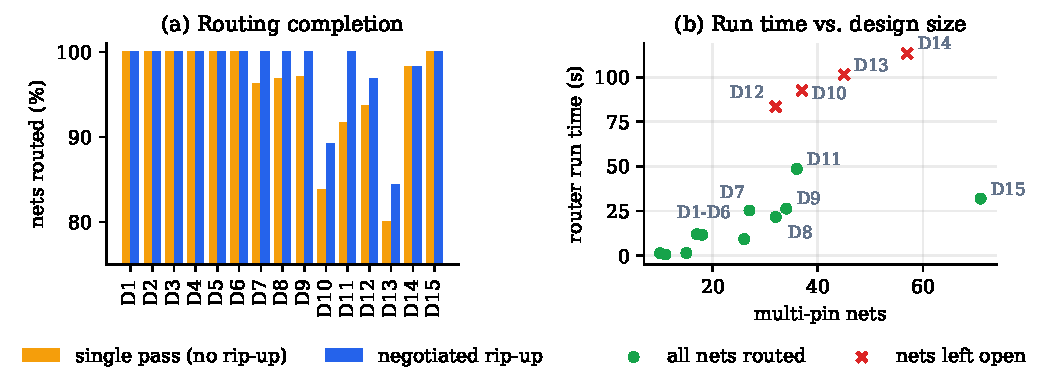
\includegraphics[width=0.92\textwidth]{figs/routing.pdf}
\caption{(a) Share of nets routed per design without and with the negotiated rip-up loop. (b) Router run time against design size for the full router; red crosses mark designs that kept open nets after the 60\,s negotiation budget and the closure passes.}
\label{fig:routing}
\vspace{-3mm}
\end{figure*}

\textbf{Routing.} Table~\ref{tab:routing} and Fig.~\ref{fig:routing} give the results. The full router completed \FullOk{} of \DesignCount{} boards and \NetsFull{} of \NetsAll{} nets; without rip-up, \NoRipOk{} boards and \NetsNr{} nets were completed. The single pass suffices on the sparse single-sided and small boards, where both variants produce identical copper. The negotiation loop matters on the dense two-layer wearables, where the first pass routinely leaves one to three nets blocked and the loop recovers them at the cost of a few extra vias. Run time grows with board density more than with net count: the single-sided CNC boards route in about a second, the 0.05\,mm-grid wearables in 10--50\,s, and boards that do not converge consume the whole budget. \RoutingNote{}

\textbf{Remaining errors.} The DRC errors in Table~\ref{tab:routing} are of two kinds. ``Unrouted'' entries are nets the router could not complete; for each, it returned the blocked pads and a suggestion, which in interactive use leads the agent to \tool{optimize\_pcb} or to a placement change. ``Via-in-pad'' entries come from vias allowed as a last resort when a pin is boxed in. We report them as errors because the strict rule set forbids them, and the Gerber export refuses such a board until they are fixed.

\textbf{Fabrication on a desktop CNC.} Table~\ref{tab:cnc} lists the isolation-milling jobs for the two single-sided boards, with and without SMD pad relief, for a 30\textdegree{} V-bit with a 0.1\,mm tip at 0.2\,mm depth (0.207\,mm groove), two passes, 1.0\,mm drills and a 2\,mm end mill for the cutout. The verification found no short at the narrowest groove and no cut net at the widest groove in any job. Pad relief added 21 rings to D1 (each relieved pad gains its own ring) for about one extra minute of milling, and changed nothing on D2, which has no SMD pads on its pour. Fig.~\ref{fig:cnc} shows the toolpaths and both previews; the D1 board was milled on a CNC 3018 desktop machine.

\begin{table}[t]
\centering
\caption{Isolation-milling jobs (GRBL G-code). Check: shorts at the narrowest groove / nets cut at the widest groove.}
\label{tab:cnc}
\footnotesize
\setlength{\tabcolsep}{2.3pt}
\rowcolors{2}{rowgrey}{white}
\begin{tabular}{@{}llcrrrrrcr@{}}
\toprule
ID & Relief & Board & Rings & Path & Holes & Lines & Min & Check & Gen.\\
 & & (mm) & & (mm) & & & & & (s) \\
\midrule
\tabinput{tables/cnc.tex}
\bottomrule
\end{tabular}
\vspace{-2mm}
\end{table}

\begin{figure*}[t]
\centering
\begin{subfigure}[b]{0.335\textwidth}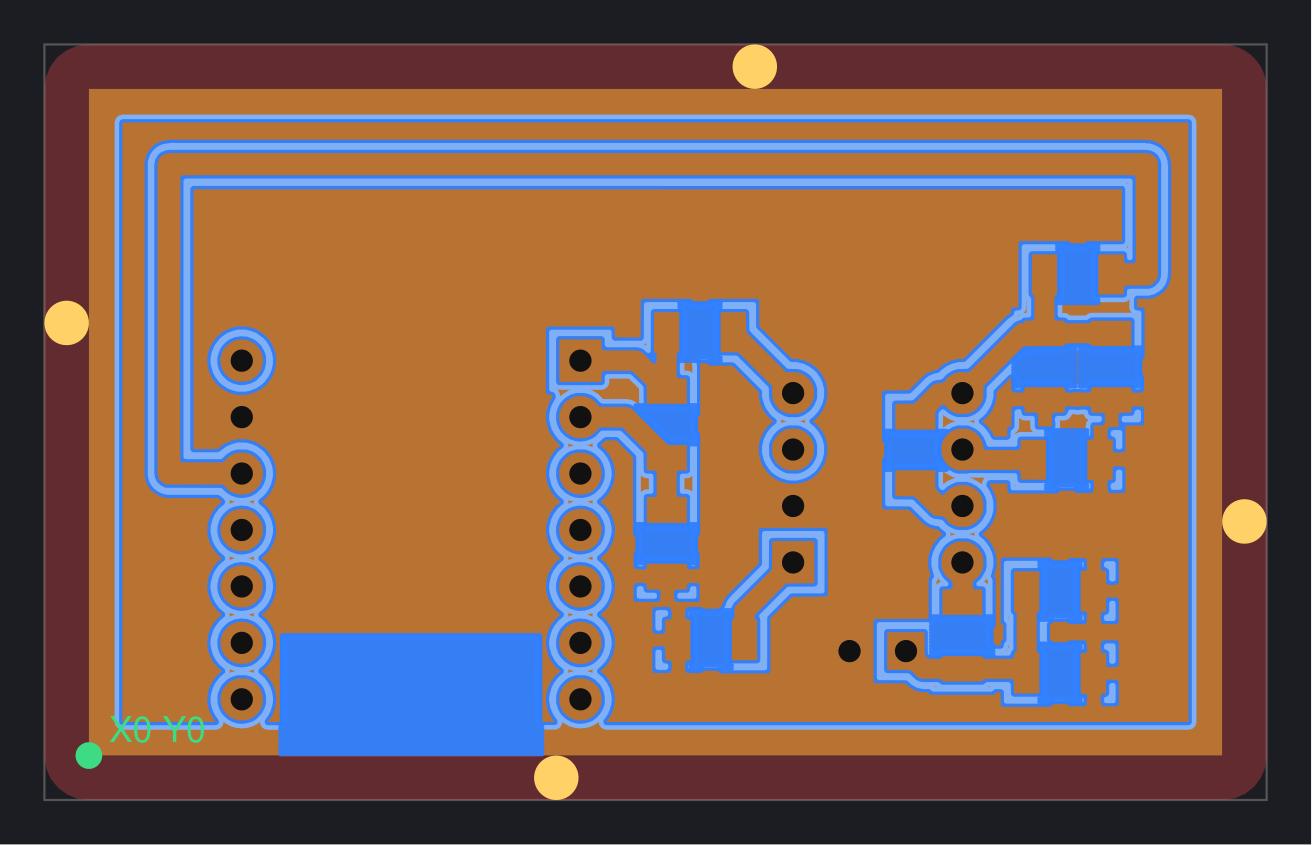
\includegraphics[width=\linewidth]{figs/cnc_paths.png}\caption{Toolpaths: isolation (blue), cutout (red), tabs (yellow)}\end{subfigure}\hfill
\begin{subfigure}[b]{0.31\textwidth}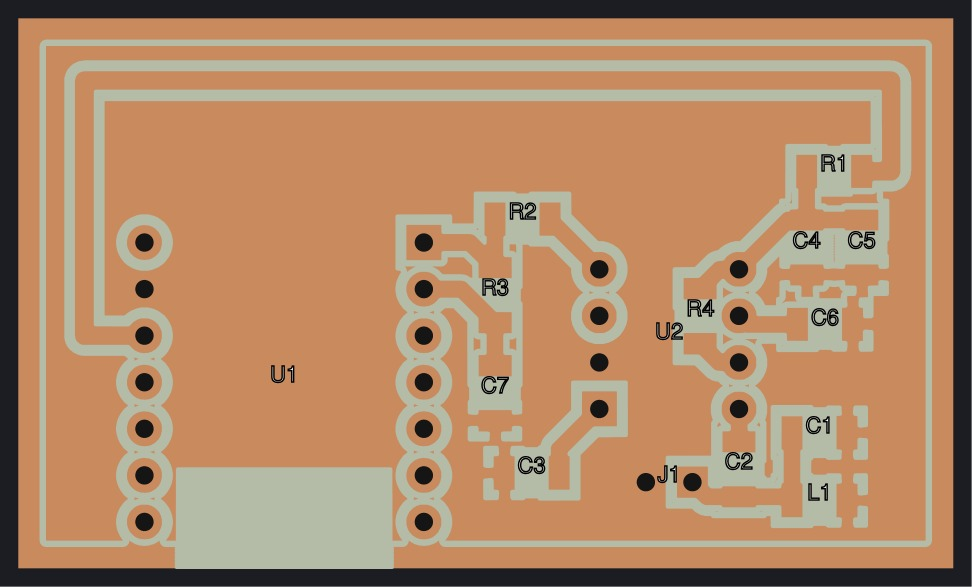
\includegraphics[width=\linewidth]{figs/cnc_2d.jpg}\caption{Result preview (2D)}\end{subfigure}\hfill
\begin{subfigure}[b]{0.32\textwidth}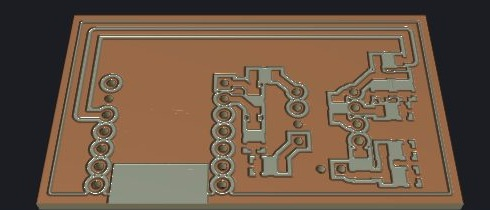
\includegraphics[width=\linewidth]{figs/cnc_3d.jpg}\caption{Result preview (3D)}\end{subfigure}
\caption{Desktop-CNC output for D1 (AD8310 log-amplifier HBC receiver on a XIAO nRF52840), generated directly from the routed board without an external CAM tool. Through-hole parts go in from the bare side, so the job is mirrored automatically.}
\label{fig:cnc}
\vspace{-3mm}
\end{figure*}

\textbf{How much state does an agent read?} Fig.~\ref{fig:tokens} compares the size of tool answers with the raw project JSON (about four characters per token). Across the \DesignCount{} designs, \tool{get\_pcb\_layout} returns \LayoutPct{} and \tool{get\_design} \DesignPct{} of the raw document; the largest board's layout answer is about \MaxLayoutTok{} tokens against \MaxRawTok{} for the raw project. The track list is the exception (\TracksPct{}), which is why it is filtered by default (\texttt{near}, \texttt{region}, \texttt{vias\_only}). The tool definitions themselves amount to about \SchemaTok{} tokens---a fixed cost that MCP clients pay once per session.

\begin{figure}[t]
\centering
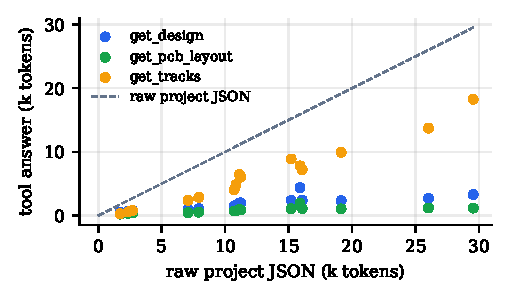
\includegraphics[width=\columnwidth]{figs/tokens.pdf}
\caption{Size of tool answers against the raw project JSON for the \DesignCount{} designs. Points below the dashed line save context; the layout summary stays nearly flat as designs grow.}
\label{fig:tokens}
\vspace{-3mm}
\end{figure}

\textbf{Schematic organizer.} Fig.~\ref{fig:sch} shows D1's schematic as first placed by the agent and after one click of \emph{Organize}. Measured on the wires the router draws, total wire length fell from 3580 to 2560 units ($-28\%$) and bends from 36 to 27 ($-25\%$), while crossings rose from 2 to 4: the organizer pulls each part next to its pin, which sometimes forces a crossing that a sparser layout avoided. Organizing and routing took 13--416\,ms across the \DesignCount{} designs (54\,ms for D1), fast enough to rerun on every edit. Most stored wearable designs use net labels instead of wires; organizing them converts labels to drawn wires, which makes them longer by construction, so we do not report a ``before'' figure for those.

\begin{figure*}[t]
\centering
\begin{subfigure}[b]{0.37\textwidth}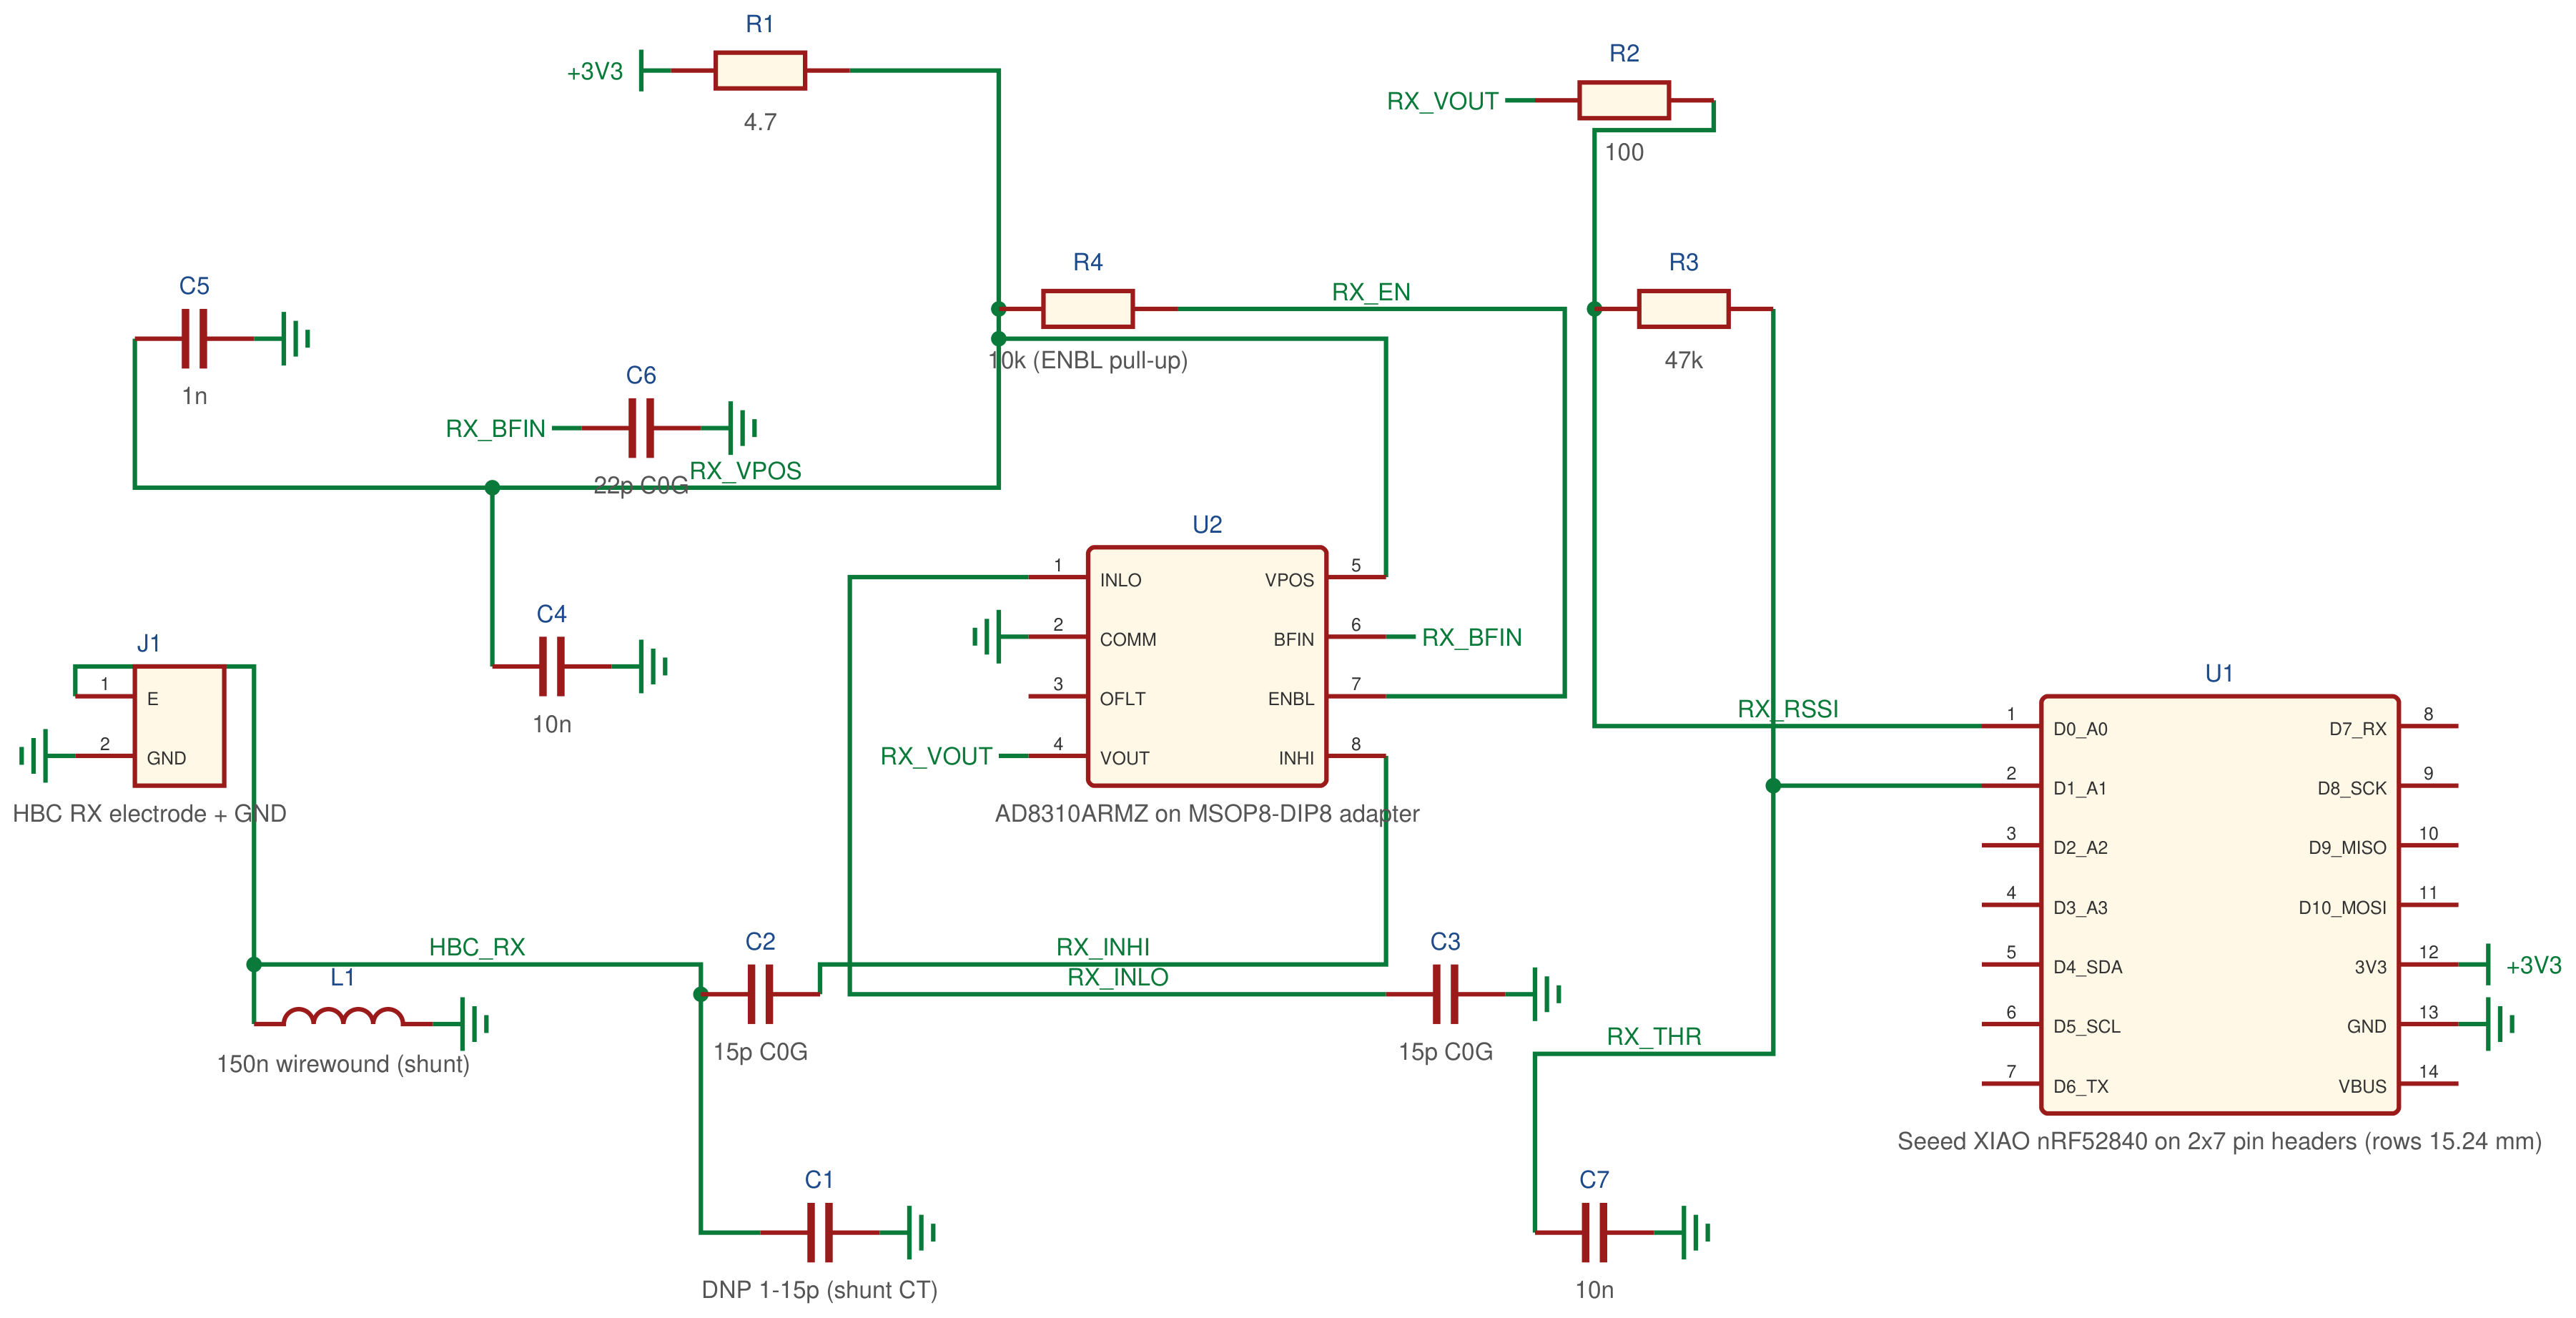
\includegraphics[width=\linewidth]{figs/sch_before.png}\caption{As placed by the agent}\end{subfigure}\hfill
\begin{subfigure}[b]{0.61\textwidth}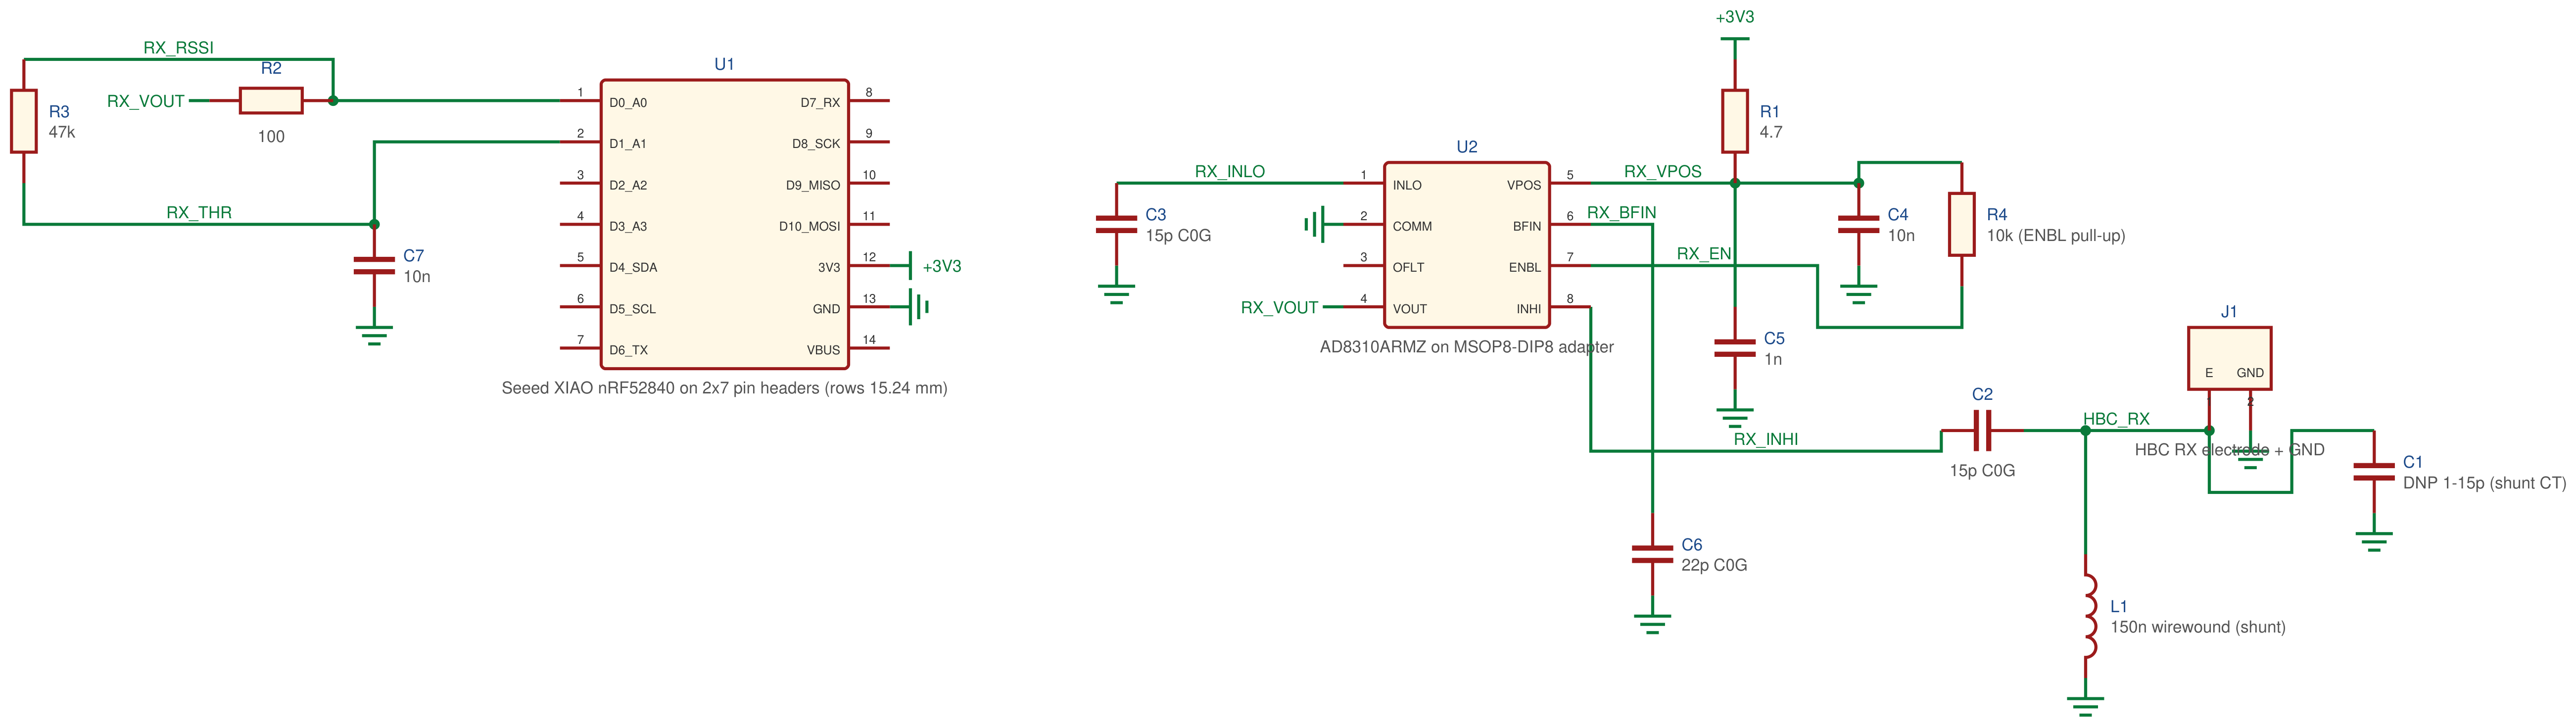
\includegraphics[width=\linewidth]{figs/sch_after.png}\caption{After \emph{Organize}: parts beside their pins, ground down, supply up}\end{subfigure}
\caption{Schematic of D1 (AD8310 receiver) before and after the organizer.}
\label{fig:sch}
\vspace{-3mm}
\end{figure*}

\textbf{End-to-end case study.} Fig.~\ref{fig:app} shows the application with the copilot, and Fig.~\ref{fig:case} shows a 49-part nRF52832 sensor node on a 26$\times$24\,mm two-layer board (37 nets, 101 vias, fully routed) and the wearable enclosure generated for the HBC node. Starting from a natural-language request, the agent selected parts with exact LCSC pinouts, wired the schematic, generated and routed the board, and produced Gerber, BOM and pick-and-place files for assembly at JLCPCB, an STL enclosure for multi-jet-fusion printing and a product datasheet. Where the user disagreed with a decision, they changed it through the same tools, and the agent continued from the edited design.

\begin{figure*}[t]
\centering
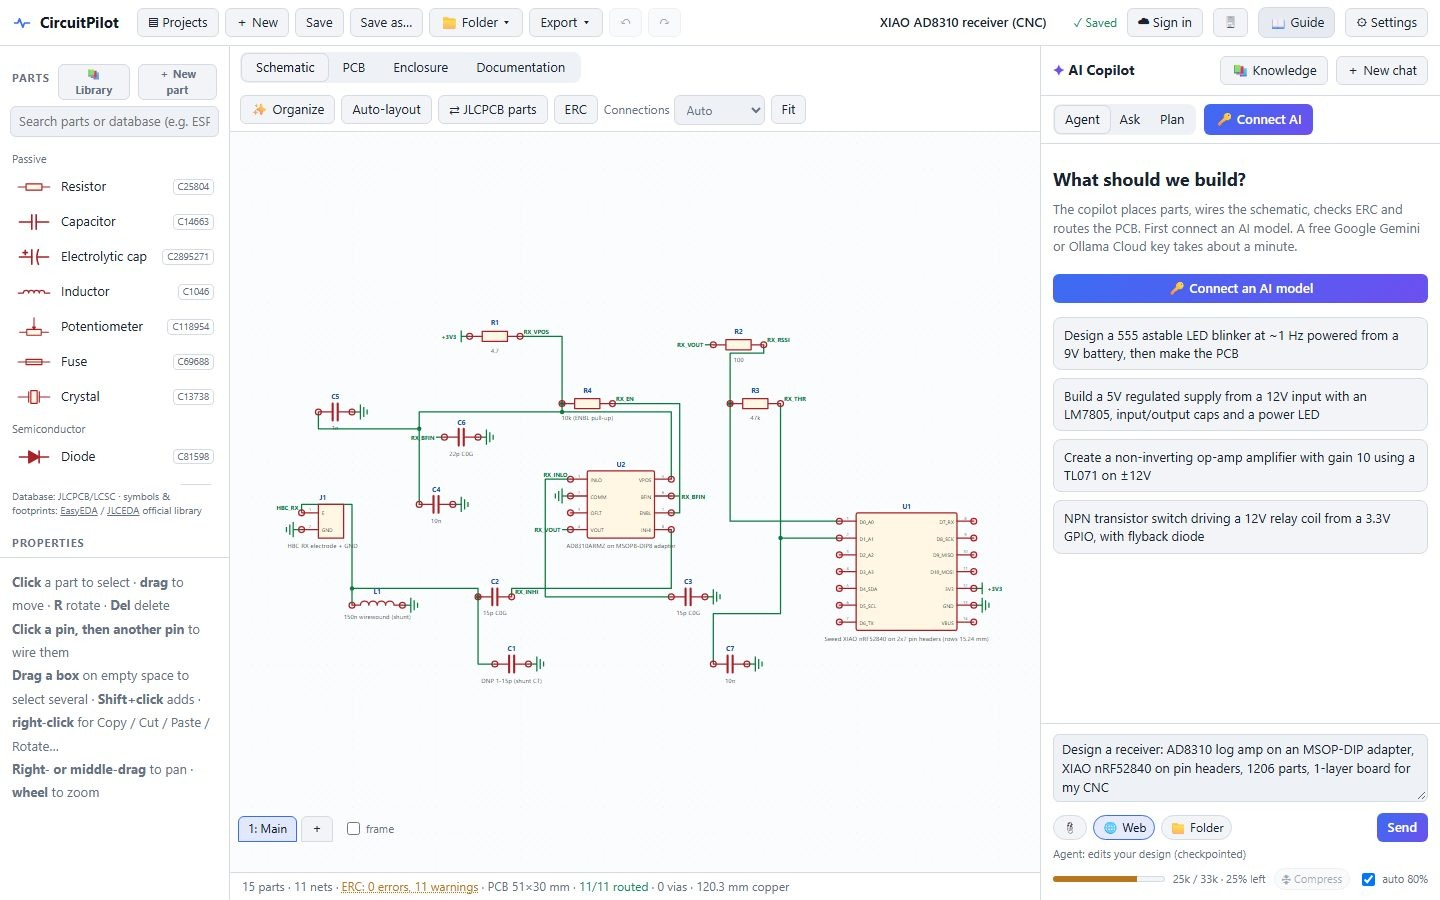
\includegraphics[width=0.86\textwidth]{figs/app_overview.jpg}
\caption{The CircuitPilot web application: parts library (left), schematic editor (centre) and AI copilot (right). The same editors serve the PCB, enclosure and documentation views.}
\label{fig:app}
\vspace{-3mm}
\end{figure*}

\begin{figure*}[t]
\centering
\begin{subfigure}[b]{0.27\textwidth}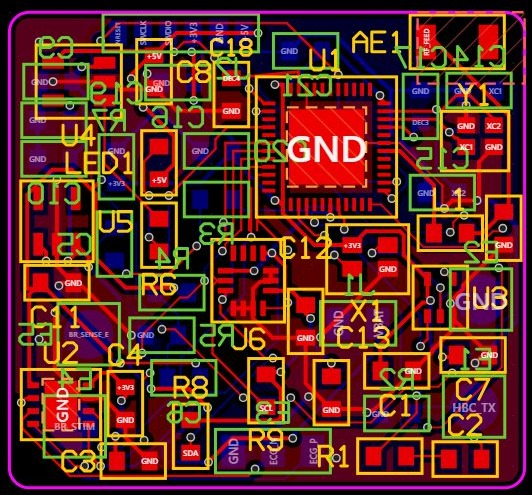
\includegraphics[width=\linewidth]{figs/pcb_2d.jpg}\caption{Routed board (top red, bottom blue)}\end{subfigure}\hfill
\begin{subfigure}[b]{0.39\textwidth}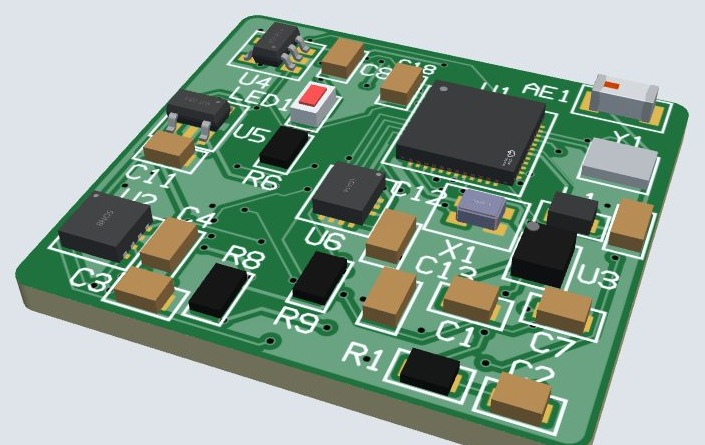
\includegraphics[width=\linewidth]{figs/pcb_3d.jpg}\caption{3D view with supplier 3D models}\end{subfigure}\hfill
\begin{subfigure}[b]{0.27\textwidth}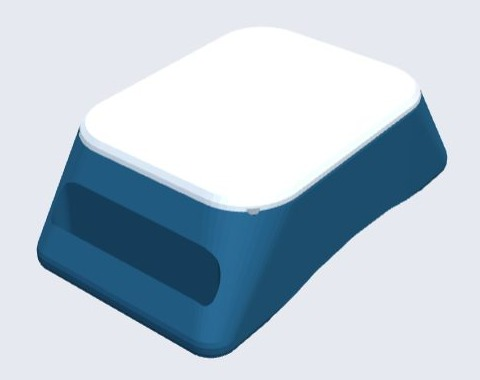
\includegraphics[width=\linewidth]{figs/enclosure.jpg}\caption{Generated wearable enclosure}\end{subfigure}
\caption{End-to-end results: a 26$\times$24\,mm nRF52832 sensor node (49 parts, 37/37 nets routed) and a 3D-printable enclosure for the HBC wearable node.}
\label{fig:case}
\vspace{-3mm}
\end{figure*}

% ============================================================
\section{Discussion and Limitations}
\label{sec:disc}

\textbf{What the split buys.} Because geometry comes only from engines, an agent's mistakes are confined to intent: a wrong part, a wrong connection, a poor rule choice. These are visible in ERC, DRC and the rendered views, and they are reversible through versions. In the other direction, engine failures are worded for the agent, so a failed route becomes a next action instead of a dead end.

\textbf{Limitations.} (i)~The router is grid-based and limited to two copper layers; it has no length matching, differential pairs or impedance control, so it targets low-speed mixed-signal boards rather than high-speed designs. (ii)~Its search is randomised within a time budget, so dense boards may finish differently between runs; the reported numbers are from single runs. (iii)~The benchmark comes from one project family and one designer, and the placements were made in the loop with the tool, which may favour it; a comparison with Freerouting on exported DSN files, and placement-from-scratch experiments, are future work. (iv)~We have not run a controlled user study; claims about accessibility are from use, not from measurement. (v)~The organizer improves wire length and bends but can add crossings. (vi)~Agent behaviour depends on the model used; we did not benchmark models against each other here. (vii)~CircuitPilot is source-available under the PolyForm Strict 1.0.0 licence (noncommercial use, no modification); versions up to v2026.10.30.6 remain Apache-2.0.

\textbf{Future work.} Model-to-model comparisons on a shared task set, integration with public PCB benchmarks~\cite{song2026pcbworld,lu2026omnilayout}, a user study with non-specialist researchers, and routing beyond two layers.

% ============================================================
\section{Conclusion}
CircuitPilot shows that a language-model agent can carry a design from a sentence to a manufacturable board when the work is divided correctly: the model decides, and deterministic, explainable engines produce and verify the geometry. A single engine shared by the browser, a static site, a desktop application and an MCP server gives agents \ToolCount{} tools with compact answers and actionable failures. On \DesignCount{} real boards, negotiated rip-up completed \FullOk{} boards against \NoRipOk{} for a single pass, and desktop-CNC jobs were generated with verified toolpaths and previewed before milling. The tool is available at \url{https://pcbgo.site}.

\section*{Availability}
The application runs in the browser at \url{https://pcbgo.site}; source code, the benchmark scripts (\texttt{docs/paper/bench}) and a 33-page tutorial are at \url{https://github.com/Abdelhayali/CircuitPilot}.

\section*{Acknowledgment}
Parts of the software and of this manuscript were developed with the assistance of AI coding and writing tools. The author reviewed all content and is responsible for it.

\balance
\bibliographystyle{IEEEtran}
\bibliography{refs}

\end{document}
